\documentclass[12pt]{report}

\usepackage{amssymb}
\usepackage{amsmath}
\usepackage{amscd}
\usepackage{amsthm}
\usepackage[utf8]{inputenc}
\usepackage[spanish,mexico]{babel}
\usepackage{enumerate}
\usepackage[usenames]{color}
\numberwithin{section}{chapter}

\usepackage{pgf,tikz}
\usetikzlibrary{arrows}

\usepackage{multicol}

\usepackage{graphicx}
\usepackage{subfigure}

\usetikzlibrary{knots,hobby,decorations.pathreplacing,shapes.geometric,calc}
\tikzset{knot diagram/every strand/.append style={ultra thick,red}, show curve controls/.style={postaction=decorate, decoration={show path construction, curveto code={\draw [blue, dashed](\tikzinputsegmentfirst) -- (\tikzinputsegmentsupporta) node [at end, draw, solid, red, inner sep=2pt]{}; \draw [blue, dashed] (\tikzinputsegmentsupportb) -- (\tikzinputsegmentlast) node [at start, draw, solid, red, inner sep=2pt]{} node [at end, fill, blue, ellipse, inner sep=2pt]{};}}}, show curve endpoints/.style={ postaction=decorate, decoration={show path construction, curveto code={\node [fill, blue, ellipse, inner sep=2pt] at (\tikzinputsegmentlast) {};}}}}



\usepackage[colorlinks=true, linkcolor=blue, urlcolor=red,
citecolor=green]{hyperref}

\voffset=-2cm
\hoffset=-3cm
\textwidth = 19.5cm
\textheight= 23 cm

\usepackage{iwona}
\usepackage{fancyhdr}
\pagestyle{fancy}
\fancyhf{}
\fancyhead[RE,LO]{\bfseries{Seminario de Topología B}}
\fancyhead[LE,RO]{\bfseries{2019-2}}
\fancyfoot[RE,RO]{\bfseries{Febrero 2019}}
\fancyfoot[LE,LO]{\bfseries{Tarea 01}}

\newcommand{\R}{\mathbb R}
\newcommand{\Q}{\mathbb Q}
\newcommand{\E}{\mathbb E}
\newcommand{\s}{\mathbb S}
\newcommand{\C}{\mathbb C}
\newcommand{\F}{\mathbb F}
\newcommand{\T}{\mathbb T}
\newcommand{\p}{\mathbb P}
\newcommand{\I}{\mathbb I}
\newcommand{\A}{\mathbb A}


\begin{document}
\begin{center}
\textcolor{blue}{\textbf{\large Guía de ejercicios para al Evaluación Parcial 01}}\\
\vspace{0.5 cm}
\textcolor{red}{\textbf{\large EXAMEN PARCIAL 01 \\ VIERNES
08-MARZO-2019\\ De 19:00 a 21:00 HORAS - Salón P-108}}
\end{center}

\begin{enumerate}
\item Demostrar que todo nudo poligonal tiene una proyección regular.

\item Esbozar un diagrama de los siguientes nudos:
%\begin{multicols}{3}
\begin{enumerate}
\item $T_{4,5}$.
\item $c(3,8)$.
\item $l(2,-7)$.
\end{enumerate}
%\end{multicols}

\item Esbozar un diagrama del nudo $T_{2,3}$ y del nudo $T_{3,2}$ para dar explícitamente la sucesión de movimientos de Reidemeister que muestran que equivamentes.

\item Demostrar que $T_{p,q}$ tiene una proyección con $p(q-1)$ cruces.

\item Demostrar que la $5$-coloración es un invariante en el conjunto de diagramas de nudos.

\item Esbozar un diagrama del nudo satelital del nudo ocho, encajado como indica la figura, que tenga como corazón al nudo $T_{3, 5}$.
\begin{center}
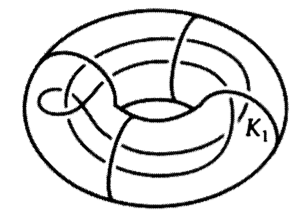
\includegraphics[width=0.75\textwidth] {05.png}
\end{center}

\item Encontrar un nudo que no sea $3$-coloreable ni $5$-coloreable.

\item Determinar una sucesión de movimientos de Reidemeister que muestren si los siguientes nudos son equivalentes.
\begin{center}
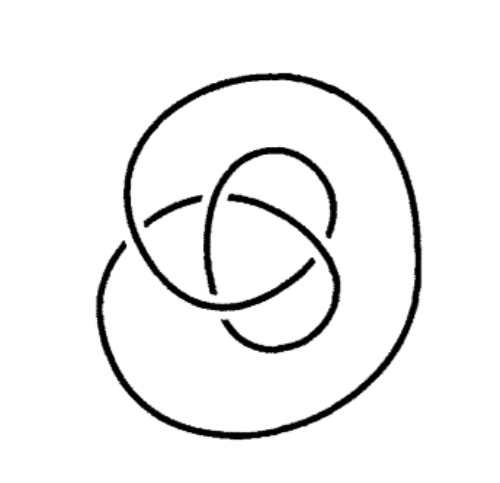
\includegraphics[width=0.4\textwidth] {04.png}\quad
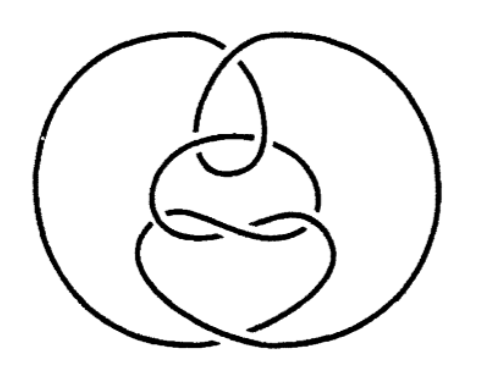
\includegraphics[width=0.4\textwidth]{01.png}
\end{center}

\item Determinar la $p$-coloración de los siguientes nudos:
\begin{center}
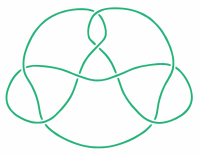
\includegraphics[width=0.4\textwidth] {02.png}\quad 
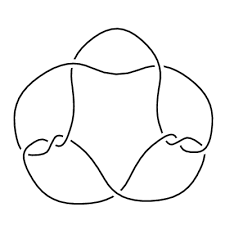
\includegraphics[width=0.4\textwidth] {03.png}
\end{center}

\item Demostrar que la suma conexa de dos nudos $3$-coloreables es un nudo $3$-coloreable.
\end{enumerate}
\end{document}